\section{Dart applications}

Creating a Flutter application can be done easily through the command line interface. 
To initiate a new application, use the following command:
\begin{verbatim}
    flutter create app_name
\end{verbatim}
This command generates a directory structure containing various subdirectories and files. 
Some of these subdirectories contain auto-generated code for different platforms, while others are critical for development:
\begin{itemize}
    \item \texttt{lib} directory: this folder holds all the handwritten code for your application.
    \item \texttt{pubspec.yaml} file: this file serves as the application's table of contents. 
        It is used to import external libraries and declare dependencies.
\end{itemize}
To run the application, execute the command:
\begin{verbatim}
    flutter run
\end{verbatim}
This command allows you to choose the platform on which you want to run the application. 
If certain platforms are unavailable on your development device, Flutter will emulate the desired device. 

Initially, the \texttt{lib} directory contains a file named \texttt{main.dart}, which includes the following code:
\begin{verbatim}
import 'package:flutter/material.dart';
    
void main() {
    runApp();
}
\end{verbatim}
Depending on the desired look and feel, you can import either \texttt{material.dart} for Material Design or \texttt{cupertino.dart} for iOS-style components. 
The \texttt{main} function contains the \texttt{runApp} method, which initializes the application.

The \texttt{runApp} function takes a given Widget and sets it as the root of the widget tree. 
This tree typically consists of two widgets: the Center widget and its child, the Text widget.
The Flutter framework ensures that the root widget covers the entire screen.

\subsection{Functions}
In Dart, a function can have any number of required positional parameters, which may be followed by either named parameters or optional positional parameters, but not both simultaneously. 
Named parameters are optional unless explicitly marked as required. 
You can also define default values for both named and positional parameters using the equals sign (=). 
These default values must be compile-time constants, and if no default value is provided, it defaults to null.

\subsection{Commas}
It is a best practice to always add a trailing comma at the end of a parameter list—this applies to functions, methods, and constructors where maintaining formatting is important. 
Adding trailing commas helps the automatic formatter insert the appropriate amount of line breaks, ensuring your code adheres to Flutter's styling guidelines.

\subsection{Widgets}
The structure of a Flutter application is fundamentally composed of widgets, which are the building blocks of the user interface. 
The following figure illustrates the material design structure used in Flutter applications:
\begin{figure}[H]
    \centering
    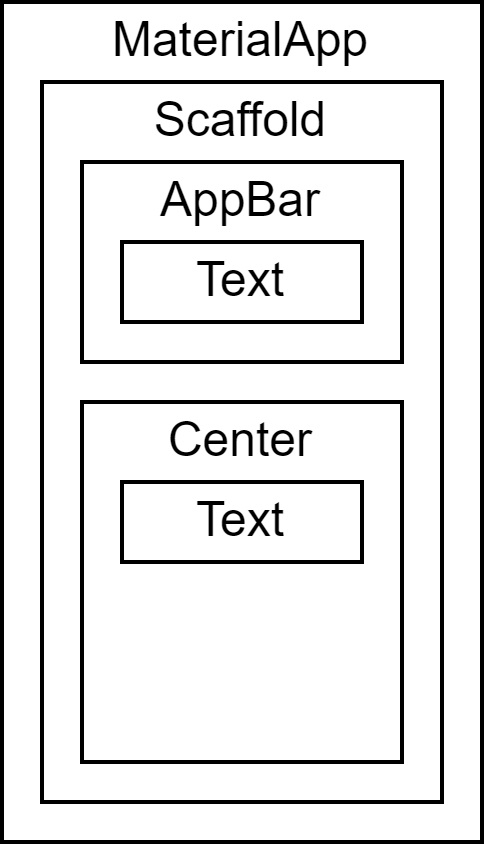
\includegraphics[width=0.5\linewidth]{images/material.png}
    \caption{Material structure}
\end{figure}
In Flutter, graphical user interfaces (GUIs) are created entirely through code, where nearly everything is represented as a widget. 
Key characteristics of widgets include:
\begin{itemize}
    \item \textit{Immutability}: a widget is an immutable object, meaning that once it is created, its properties cannot be changed. 
        Instead, to modify a widget's appearance or behavior, a new widget must be created.
    \item \textit{Composability}: widgets are composable, allowing developers to combine existing widgets to build more complex interfaces. 
        This enables the creation of new widgets by composing smaller, reusable ones.
    \item \textit{Descriptive nature}: widgets describe what the GUI should look like. 
        They provide a visual representation of the interface and its components.
\end{itemize}
When the state of a widget changes, the Flutter framework responds by rebuilding the affected widget. 
The framework performs the following steps:
\begin{enumerate}
    \item \textit{Diff computation}: it computes the difference between the current widget state and the previous rendering, determining what has changed.
    \item \textit{Minimal changes}: the framework identifies the minimal set of changes needed to update the interface, optimizing performance.
    \item \textit{Selective re-rendering}: only the parts of the UI that have changed are re-rendered, which enhances efficiency and responsiveness.
\end{enumerate}
This architecture of widgets allows for flexible and dynamic user interfaces that can easily adapt to user interactions and data changes.

All widgets have a state, which can be categorized as either mutable or immutable.
The state of a stateful widget is changeable; for example, it may represent the current position of a slider or whether a checkbox is checked. 
This state is stored in a State object, allowing for a clear separation between appearance and content. 
To update the appearance of the widget in response to changes, we need to call \texttt{setState}, which informs the framework to redraw the widget.

In contrast, a stateless widget does not manage any internal state. 
Stateful widgets maintain state that can change, allowing them to alter their appearance based on user events or incoming data. 
Implementing a stateful widget requires two classes: one that extends \texttt{StatefulWidget} and another that defines the mutable values and includes the \texttt{build} method to render the widget.

\paragraph*{Const and final}
In Dart, the keyword \texttt{const} is used for values known at compile time (e.g., \texttt{const a = 1}), while \texttt{final} is appropriate for values that are determined at runtime. 
Anything not known at compile time should be declared as \texttt{final} instead of \texttt{const}.

\paragraph*{State management}
The \texttt{setState} method notifies Flutter of a state change, prompting the widget to be re-rendered. 
This triggers the re-execution of the \texttt{build} method, ensuring the GUI reflects any updates. 
If the state variable (e.g.,\texttt{\_counter}) is modified without invoking \texttt{setState}, the \texttt{build} method will not be called, and the GUI will remain unchanged.

\paragraph*{Flexible}
The \texttt{Flexible} widget allows for resizable elements within the layout.
Unlike inflexible widgets, which are fixed in size, flexible widgets adjust according to their properties: \texttt{flex} and \texttt{fit}. 
The \texttt{fit} property dictates whether the widget occupies extra space, with \texttt{FlexFit.loose} using the widget's preferred size by default, and \texttt{FlexFit.tight} enforcing the widget to fill all available space. 
The \texttt{flex} property defines the resize ratio relative to other widgets.

\paragraph*{Other options}
The \texttt{Expanded} widget can wrap a widget, compelling it to fill any available extra space.
Conversely, \texttt{SizedBox} can wrap a widget and resize it using specified height and width properties; it can also create empty space by setting these dimensions. 
The \texttt{Spacer} widget generates space between widgets, utilizing the flex property, while \texttt{SizedBox} provides space based on a specific number of logical pixels.

\subsection{Assets}
To incorporate external assets, they must be explicitly declared in the project. 
To include all assets within a directory, use the directory name followed by a slash (e.g., \texttt{assets/}). 
If assets are located in subdirectories, each directory must have a separate entry in the asset declaration.